\section{Memoria del proyecto}
\label{memoria}
A continuación se describen los objetivos principales de cada uno de los equipos de trabajo así como un pequeño resumen de cómo se ha desarrollado el trabajo de cada equipo a lo largo de todo el proyecto. En el resto de la sección se describe más detalladamente el desarrollo del proyecto.\\

\subsubsection*{FrontEnd y Middleware}
El principal objetivo del Frontend eran desarrollar las interfaces con las que los usuarios interaccionarían con la aplicación. Se distinguen dos interfaces, las de navegación web y la parte jugable del guiñote. La parte jugable se ha podido implementar en su mayoría, a falta del modo espectador y la parte de personalización. Para la segunda interación se realizaron los torneos, integración de la IA, espectadores y resto de vistas web, junto con las del administrador.
\\
En cuanto al Middleware, el principal objetivo era comunicar la interfaz de juego para que los usuarios puedan jugar entre ellos, gracias al paso de mensajes.

\subsubsection*{BackEnd}
El objetivo del equipo backend era desarrollar un paquete de java que representase la lógica del juego del guiñote, al mismo tiempo que desarrollaba gran parte de la página web dinámica del proyecto. Sin embargo, a mitad de desarrollo el trabajo, se centró en acabar la parte de la lógica del juego. Dicho objetivo se ha cumplido completamente con algunos retrasos en la entrega. Como consecuencia la web dinámica arrastra un leve retraso que deberá ser compensado en la segunda iteración. A pesar de dichas dificultades el equipo ha trabajado mucho para conseguir una primera versión funcional antes de la primera iteración.

\subsubsection*{Base de datos}
Los principales objetivos del equipo de bases de datos eran por una parte diseñar e implementar la base de datos para el sistema (esquema conceptual, lógico y físico) y por otra desarrollar la capa de acceso a datos proporcionando una interfaz para el Backend. Ambos objetivos se cumplieron en su totalidad y según el plazo establecido, a excepción de los torneos, que debido a su complejidad (no estimada en un primer momento) se alargó su desarrollo varias semanas. Además, el equipo desarrolló los eventos periódicos de la base de datos: torneos periódicos y actualización de ligas. Exceptuando las pequeñas dificultades iniciales relacionadas con un tardío diseño de la interfaz de acceso a datos, tanto la comunicación entre los miembros del equipo como con el resto de equipos se ha desarrollado sin problemas. En la parte final de integración, se detectaron algunos errores en el acceso a datos, aunque la depuración de esta parte de la aplicación fue una de las menos complejas y fueron solucionados todos los errores sin mayores problemas. El trabajo del equipo en general ha sido muy satisfactorio. 

\subsubsection*{Inteligencia Artificial}
El objetivo del equipo de inteligencia artificial ha sido cumplido con un claro éxito: desarrollar una ia competente para jugar al guiñote 1 vs. 1. El trabajo de este equipo ha consistido en primer lugar en investigar en la literatura para aprender sobre algoritmos de inteligencia artificial utilizados en juegos similares, la decisión del algoritmo a utilizar, el desarrollo de un prototipo funcional para estudiar su viabilidad, y finalmente su implementación final y la integración de este con el resto de la aplicación. El trabajo se ha desarrollado sin problemas destacables, a excepción de que la fase de análisis e investigación fue algo más costosa de lo planificado. Los resultados de SophIA han sido mucho mejores de lo esperado, suponiendo esta una de las características más distintivas de la aplicación final.

Como decisión importante, destaca que tras un análisis del progreso del proyecto y adecuación a la planificación, el equipo de Bases de Datos iba más avanzado y tenía mucha menos carga de trabajo de cara a la segunda iteración que los equipos de BackEnd y FrontEnd. Por ello, antes de que los miembros del BackEnd comenzaran a trabajar en la Inteligencia Artificial (como así estaba decidido en un principio) se decidió reconfigurar el equipo de Inteligencia Artificial y que pasaran a formar parte de él los miembros del de Bases de Datos, con una organización final como la que se muestra en el organigrama de la sección \ref{organiz}.

\subsubsection*{IA}
El objetivo del equipo de la IA era desarrollar una inteligencia artificial capaz de tomar decisiones inteligentes a la hora de jugar al guiñote en partidas individuales. A la hora de desarrollar la IA, se decidió realizar primero un prototipo en Phyton para verificar la eficacia del algoritmo que trata el problema. Mediante una recopilación de estadísticas se determinó que el algoritmo elegido cumplía con el objetivo y se procedió a implementarlo en java.
El equipo que formaba la IA fue reconfigurado antes de empezar a trabajar añadiendo a los miembros del equipo dedicado a la base de datos dado que iban avanzados y tenían una menor carga de trabajo.

\subsection{Inicio del proyecto}
\label{Inicio del proyecto}
Tal y como se describió, tras un diseño preliminar del sistema en general, cada subequipo se puso a analizar sus necesidades concretas y a buscar ejemplos para comenzar a implementar con cierto contexto. Cabe destacar que entre las búsquedas de esos ejemplos, se estableció contacto con Iván López Asín, desarrollador de la app guiñotepro.es. Fue una sorpresa que usase generalmente las mismas tecnologías que las propuestas preliminarmente (Phaser.io y WebView para móviles), lo que resalta un buen trabajo de documentación previo del equipo. Además, mostró su interés en integrar nuestra  inteligencia artificial, pero habría que portarla a Javascript y adaptarla a su implementación, lo que se analizará y negociará al término de la segunda iteración.\\

Posteriormente, se configuró el repositorio en Github debidamente y como denominador común se ha utilizado la suite de IDEs de JetBrains: WebStorm para Javascript, IDEA para Java, JSP y Servlets y, por último, DataGrip para el diseño y la interacción con la base de datos.\\

Por último, antes de ponerse a implementar, cada equipo de trabajo debió pasar una fase de formación. Sin embargo, se ha intentado centrar la atención exclusivamente en las tecnologías que afectasen directamente a cada equipo para reducir el tiempo invertido en esto. Por suerte, el backend del proyecto está desarrollado en Java, tecnología en la que todo el mundo tiene cierta experiencia, haciendo así más fácil la interacción entre los diferentes componentes y la depuración de errores.\\

Respecto al aprendizaje de las nuevas tecnologías aplicadas en el proyecto, la experiencia ha sido generalmente positiva. En el caso de la GUI, se ha tenido que aprender a utilizar tanto Javascript como el framework de videojuegos Phaser. Para ello, se han utilizado tutoriales tanto oficiales como de terceros. Además, entre la GUI y el gestor de mensajes la comunicación se realiza a través de websockets, por lo que ha habido que formarse tanto en la perspectiva de websockets para Javascript como para JavaEE con la API de Tomcat. En el backend, los principales problemas de integración se han debido a falta de experiencia con el flujo de trabajo del IDE, lo que era un coste temporal que no estaba calculado a priori. Por último, según lo decidido, se configuró la base de datos en MySQL dentro de Amazon Aurora (AWS), tratándose de una tecnología también novedosa para el equipo. Cabe destacar que el despliegue transcurrió sin mayores incidencias siguiendo las instrucciones provistas por Amazon. Las principales características de la base de datos utilizada para el proyecto son:

\begin{itemize}
	\item Versión Software: Aurora MySQL 5.7.12
	\item Hardware: 1 CPU, 2GB RAM
	\item Identificador de la Intancia: sotayrey-aurora
	\item Identificador del Cluster: sotayrey-cluster
	\item Identificador de la base de datos: sotayrey\_db
	\item Copia de Seguridad: Cada 30 días
\end{itemize}

Éstas se deben al requerimiento de cumplir con las limitaciones de la versión gratuita para estudiantes. Además, se ha habilitado el acceso externo para facilitar la fase de desarrollo, aunque se cerrará cuando se pase a producción. Respecto al software relacionado con la base de datos, hizo falta formación en el funcionamiento de la API JDBC, así como en la utilización de pools de conexiones con c3p0 para mejorar el rendimiento, cosa que no se había especificado anteriormente en los procesos de inicio del proyecto.

\subsection{Ejecución y control del proyecto}
\label{Ejecucion y control del proyecto}
Los procesos de control no se han llevado a cabo tal y como estipulaba el primer plan de gestión. Ya que el director del proyecto no se ha coordinado con los responsables de grupo. Sin embargo a nivel local, los responsables de grupo si han dirigido y organizado sus respectivos grupos. Además no se ha producido ninguna situación que requiera de mediación ni necesidad de intervención extraordinaria por parte de los responsables. 
Los procesos técnicos se han llevado a cabo tal y como estaban especificados en la primera versión del plan de gestión. Tanto en el apartado de pruebas como documentación. Aplicar los procesos acordados ha costado bastante por la falta de costumbre, sin embargo los ficheros fuente, pruebas y documentación obtenidos nos han permitido trabajar de forma más eficiente.
\subsubsection{Reparto del trabajo}
En un primer momento, el reparto de trabajo fue definido únicamente en relación a los equipos creados, como se detalla en la sección \ref{repartotrabajo}. Sin embargo, se detectó que este reparto, aunque necesario, era demasiado genérico y no permitía medir el progreso de forma clara. Por ello se decidió que dentro de cada equipo de trabajo se llevaría a cabo una división del trabajo en tareas o paquetes de trabajo, siguiendo la Estructura de Descomposición del Trabajo (WBS \cite{edt}). Cada paquete de trabajo corresponde a una tarea específica y claramente delimitada, como puede ser el desarrollo de una clase, y especifica un único responsable de este (no significa que sea la única persona que trabaje en él pero sí la responsable de su desarrollo). Para el control del progreso en relación a esta división del trabajo se ha utilizado el apartado Projects de GitHub, en el que cada paquete se marca con un tick cuando está finalizado y depurado.

A continuación se muestran los diagramas de paquetes desarrollados:

\begin{figure}[H]
		\hspace{-2cm}
		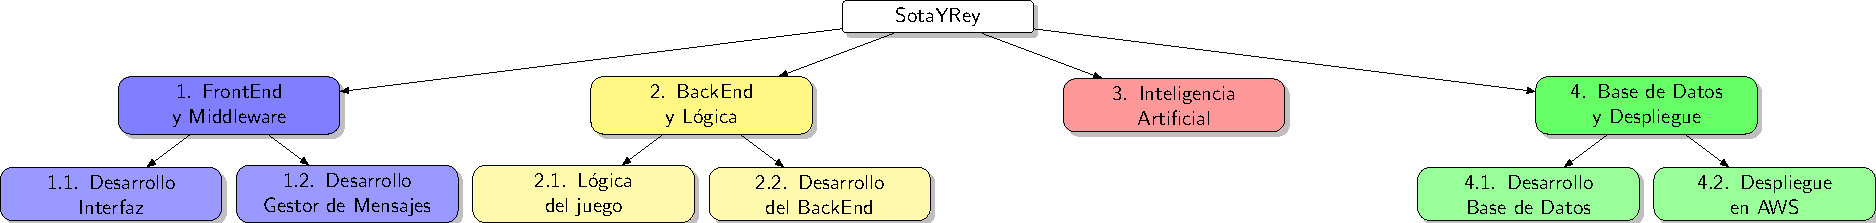
\includegraphics[scale=0.6]{figuras/edtGeneral.pdf}
		\caption{Diagrama general de reparto del trabajo}
	\end{figure}

\begin{figure}[H]
		\centering
		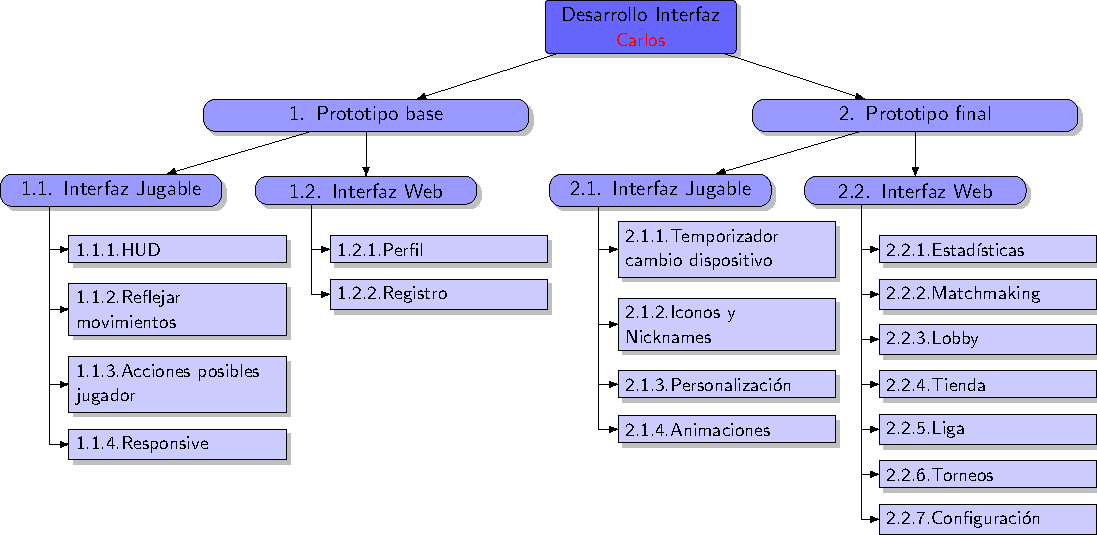
\includegraphics[scale=0.85]{figuras/edtInterfaz.pdf}
		\caption{Diagrama de Paquetes de Trabajo Interfaz}
	\end{figure}

\begin{figure}[H]
		\hspace{-2cm}
		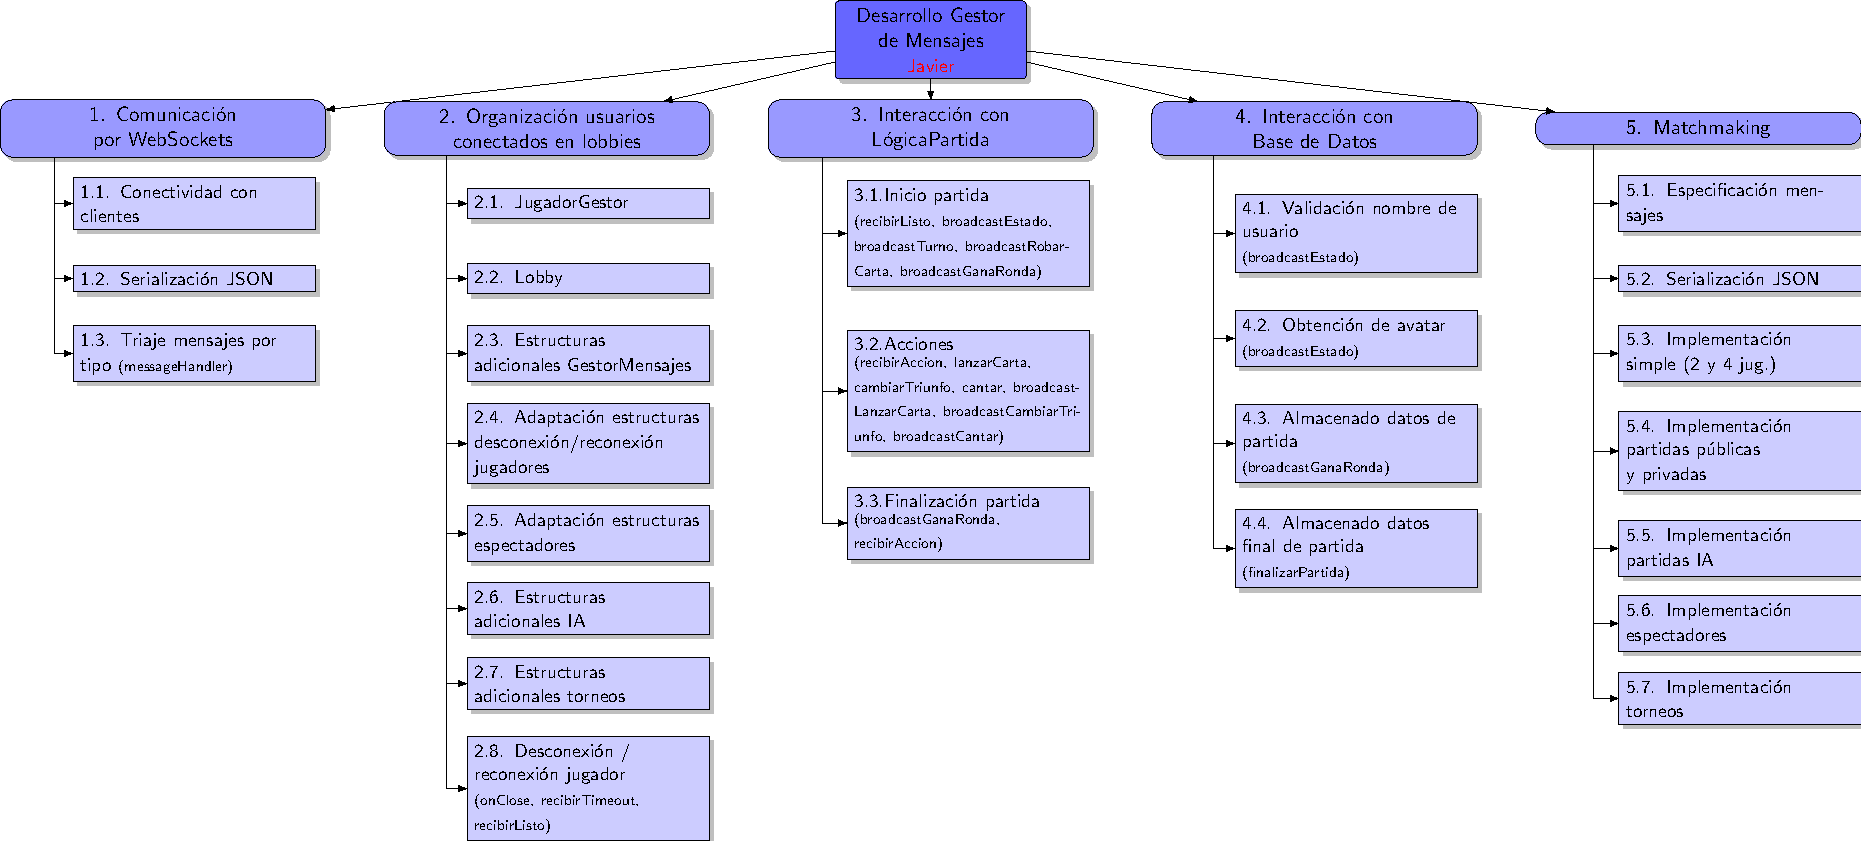
\includegraphics[scale=0.75]{figuras/edtGestorMensajes.pdf}
		\caption{Diagrama de Paquetes de Trabajo Gestor de Mensajes}
	\end{figure}


\begin{figure}[H]
		\centering
		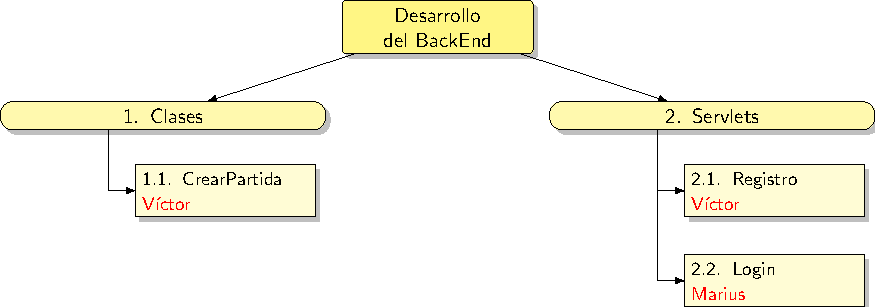
\includegraphics[scale=0.8]{figuras/edtBackend.pdf}
		\caption{Diagrama de Paquetes de Trabajo BackEnd}
	\end{figure}

\begin{figure}[H]
		\hspace{-1cm}
		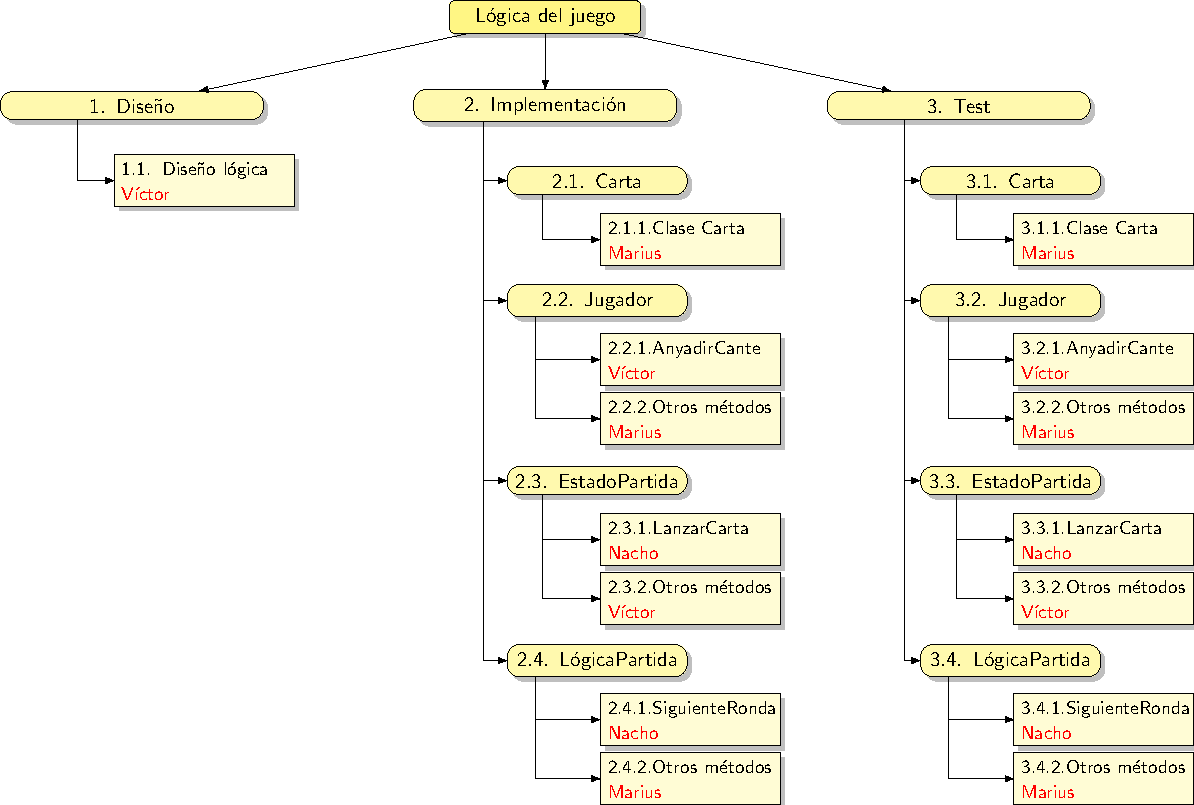
\includegraphics[scale=0.8]{figuras/edtLogica.pdf}
		\caption{Diagrama de Paquetes de Trabajo Lógica}
	\end{figure}

\begin{figure}[H]
		\hspace{-2cm}
		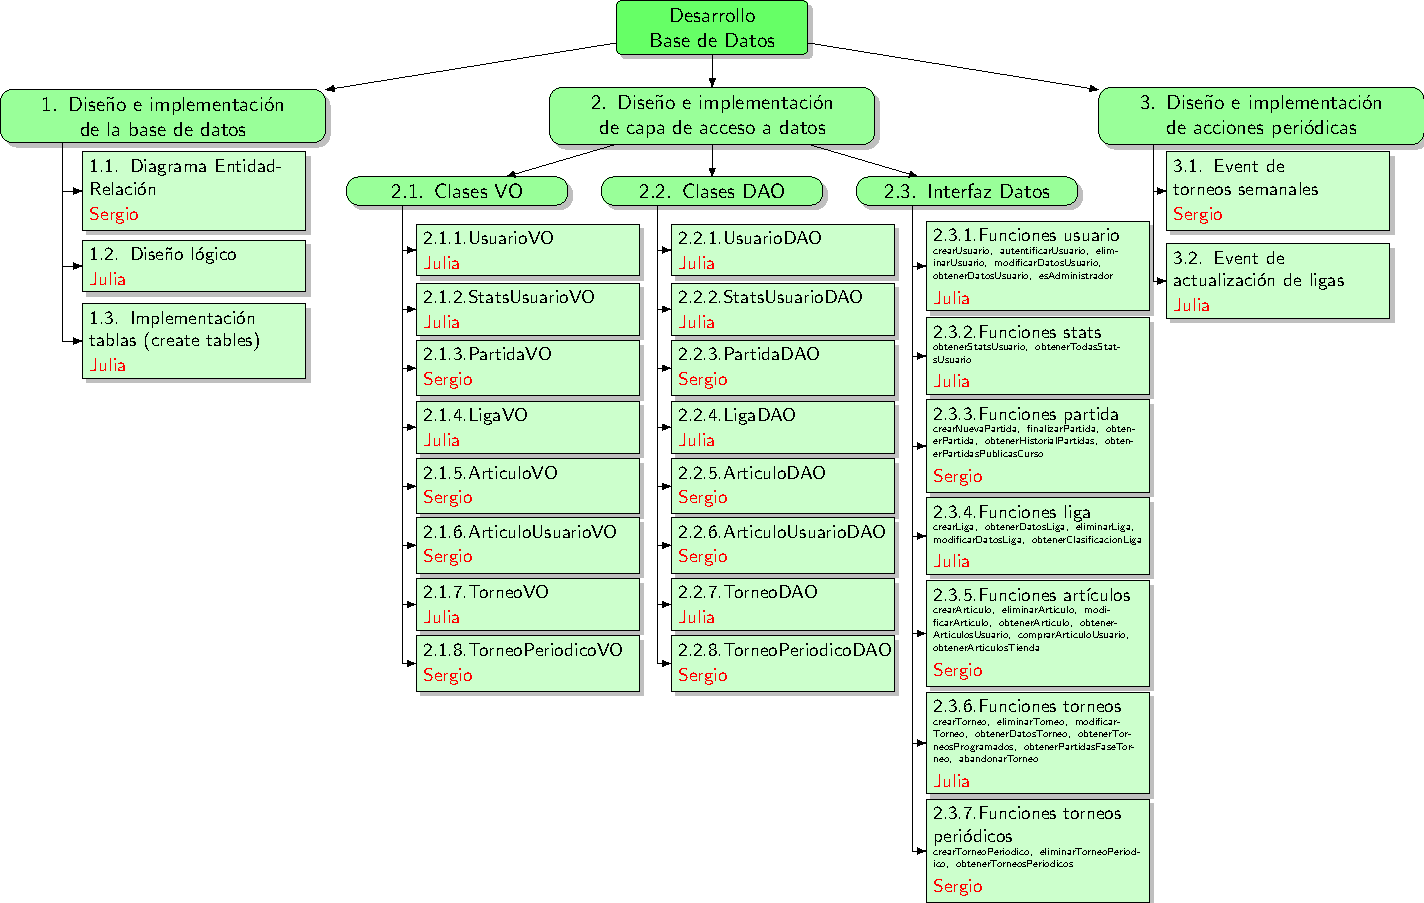
\includegraphics[scale=0.8]{figuras/edtBasesDatos.pdf}
		\caption{Diagrama de Paquetes de Trabajo Bases de Datos}
	\end{figure}

\begin{figure}[H]
		\centering
		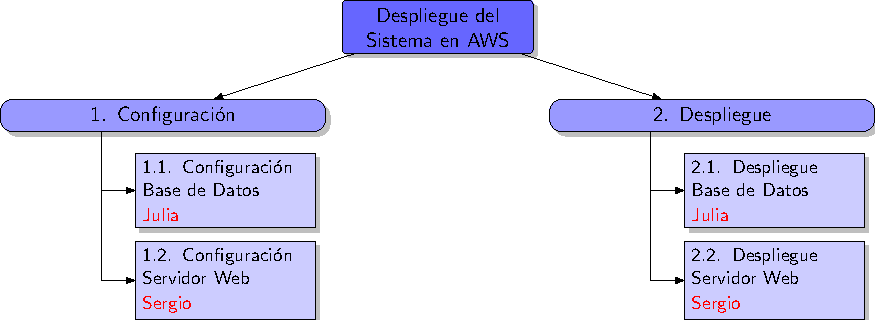
\includegraphics[scale=0.8]{figuras/edtDespliegue.pdf}
		\caption{Diagrama de Paquetes de Trabajo Despliegue}
	\end{figure}

Es importante añadir que el trabajo de integración de los diferentes paquetes de trabajo no está reflejado en estos diagramas pero también ha sido necesario repartirlo y realizarlo. A su vez, algunos de los paquetes correspondientes a la segunda iteración no se han diseñado todavía, o aunque se haya hecho, podrían producirse modificaciones sobre ellos ya que todavía no se han analizado ciertas partes a fondo.
\subsubsection{Comunicación interna}
La decisión de la nueva estructura de grupos se realizó mediante una reunión entre los miembros afectados por el cambio.
En cuanto a la parte de BackEnd, al comienzo del proyecto la comunicación ha sido bastante pobre, ya que en algunos momentos los desarrolladores han realizado la misma actividad por duplicado. En el desarrollo de los diferentes componentes cada miembro tenía su propio diseño en mente y ha sido necesario ponerse de acuerdo y plasmar el diseño en un diagrama UML de clases, que todos pudieran consultar y hacer referencia. Hacia el final de la primera iteración el equipo ha mejorado su comunicación en gran medida.
\\
La comunicación entre los diferentes equipos se ha llevado a través del servicio de terceros Skype para, principalmente, resolver dudas acerca de como comunicar e integrar las distintas partes de la aplicación. Además, se utiliza el servicio de mensajería WhatsApp para reportar bugs, incidencias y comonunicaciones asíncronas. También se han llevado a cabo varias de tipo presencial reuniones para especificar interfaces comunes para facilitar la integración
\\
Se ha utilizado Floobits para la programación por parejas para las partes de la aplicación más complejas.

\subsubsection{Adecuación a las herramientas y tecnologías}
% \subsubsection*{Base de Datos}
La base de datos se ha desplegado en el gestor elegido en un primer momento, MySQL en Amazon Aurora. Para la implementación se eligió Java como lenguaje de programación lo que ha permitido la utilización de librerias para la conexión de la base de datos (JDBC y c3p0). El desarrollo en Java fue acompañado del software IntelliJ que permitía el soporte para las librerías y el control de versiones. Además permite programar en Java, por lo que el uso de la herramienta es una ventaja.
\\

% \subsubsection*{FrontEnd y Middleware}
En cuanto al desarrollo de la interfaz de juego se ha utilizado la herramienta WebStorm, en un primer momento, ya que permite de forma fácil hacer cambios en la interfaz y verlos reflejados de manera inmediata en el navegador. Sin embargo, al integrar esta parte con el resto del proyecto se ha seguido su desarrollo con el software IntelliJ. De esta manera, se consigue probar el funcionamiento del juego gracias al despliegue con el servidor Tomcat para poder probar las comunicaciones entre jugadores.
\\
Una vez se despliegua el sistema en Amazon, para depurar las comunicaciones basta con modificar aquel fichero que se necesitaba ajustar, ya que simplemente había que ajustar parametros de retardos al tratarse de un sistema distribuido en cuanto al paso de mensajes se refiere. De esta manera no se despliega toda la aplicación de nuevo sino que sólo una parte de ella.
\\
% \subsubsection*{BackEnd}
Para el diseño de los diagramas de clases se ha utilizado la herramienta StarUML, la web draw.io y excel para los diagramas de las pruebas de caja blanca y las tablas para las pruebas de caja negra.
Se ha utilizado un plugin Floobits de Intellij para la programación en parejas ya que nos permitía trabajar remotamente a dos o más miembros sobre el mismo fichero en tiempo real utilizando dos cursores diferentes. Esta herramienta se ha utilizado para los métodos más difíciles como por ejemplo lanzarCarta de la clase EstadoPartida.
El principal problema encontrado fue que la tecnología utilizada ya que Java funciona con asociación dinámica. Todos los parámetros y tipos devueltos por las funciones son punteros. Esta característica hace que la encapsulación de los objetos desaparezca. Cuando se devuelve cualquier clase como resultado de un método, es necesario crear una replica exacta del objeto en memoria, para que el usuario no modifique los atributos privados de la clase. Por ejemplo, la clase logica\_partida debe devolver una copia exacta de su atributo interno estado\_partida con cada operación. Si en lugar de realizar una copia devuelve un puntero, un usuario externo puede modificar dicho estado con las funciones públicas de la clase estado\_partida clase.
\\
Uno de los principales problemas al trabajar con IntelliJ ha sido que el equipo olvida en ocasiones que no se debe subir el archivo de configuración, ya que incapacita al resto del equipo para trabajar y se ha de eliminar de forma manual.

\subsubsection{Control de versiones}
%\subsubsection*{FrontEnd y Middleware}
La utilización de git ha sido de gran ayuda a la hora de integrar el código desarrollado por cada miembro del grupo. Si algún miembro de un equipo modifica algún fichero de otro equipo, el commit que se realice especifica de forma clara y directa que es lo que ha modificado. Para cambios grandes se pone en contacto con el responsable del equipo para solucionar el problema. Se ha utilizado git desde el software de desarrollo intellij IDEA, en vez de hacerlo directamente sobre la línea de comandos, para subir y actualizar el proyecto de manera más rápida y cómoda. Esto ha sumado en el tiempo de aprendizaje del uso de los IDE’s.Un problema que surgió al principio del desarrollo del proyecto relacionado con el uso de git fue no realizar commits de manera frecuente, lo que provocó que algunos miembros realizarán el mismo trabajo. Para solucionarlo, se está realizando commits de manera más frecuente y se está utilizando las task lists de github para llevar un control de lo que se ha realizado o de lo que falta por realizarse o probar. Otro de los problemas encontrados consecuencia de la utilización del control de versiones fue debido a la existencia de un fichero \textit{properties} con la información privada de acceso a la base de datos, que no debía de estar subida al repositorio público. Al no existir ese fichero en un repositorio público, se tuvo que compartir de forma privada y cada usuario colocó el fichero en lugares distintos, provocando errores al compilar dependiendo de la ruta del fichero.

%\subsubsection*{Base de Datos}

%\subsubsection*{Integración y despliegue}
En cuanto a la integración entre el acceso a datos y el backend, se detectó un claro problema de comunicación entre los grupos a mitad del desarrollo debido a que no existía una interfaz definida de forma precisa desde un primer momento. Únicamente se había comentado una interfaz ambigua que diferentes partes entendían de forma distinta, y que además, sin las definiciones concretas de las funciones, impedía llevar a cabo el desarrollo en paralelo. Cuando se detectó el problema, hubo una reunión entre ambos grupos para definir esta interfaz de acceso a los datos. Gracias a este incidente se ha aprendido la importancia del desarrollo de interfaces entre los distintos componentes de los sistemas.
El despliegue del servidor de bases de datos se realizó en AWS sin mayores problemas. En cuanto al despliegue del servidor web hubo problemas debido a una configuración de red de la máquina virtual. Tras localizar el problema se pudo solventar y finalmente acceder al servidor mediante SSH sin problemas.

Para desplegar la aplicación web, se ha utilizado el servidor Tomcat en local junto con la herramienta IntelliJ. Surgieron problemas con las versiones de Tomcat por lo que hubo que adaptar el código para que funcionara en la última versión. En cuanto a la parte jugable, se despliega directamente con la herramienta WebStorm y se ejecuta en el navegador Chrome.

\subsubsection{Pruebas del software}
Para asegurar el correcto funcionamiento del software, cada equipo ha realizado pruebas unitarias para las funciones más complicadas que puedan generar errores.

%\subsubsection*{FrontEnd y Middleware}
Para probar la interfaz de juego se ha utilizado la herramienta Jasmine \footnote{ \url{https://jasmine.github.io/} }, que permite hacer tests unitarios en JavaScript. Se ha creado un protipo de una partida de prueba y se comprueba que el software pasa todos los tests diseñados.
%\subsubsection*{Bases datos}

La base de datos implementada en MySQL fue probada mediante la inserción de datos falsos de ejemplo, y la realización de consultas sencillas sobre ella, que garantizan el correcto funcionamiento. La interfaz de acceso a datos ha sido probada mediante pruebas unitarias. Se desarrolló un programa de pruebas al final del desarrollo de cada clase DAO, probando función a función sobre los datos de ejemplo introducidos, y solucionando errores de implementación. Para comprobar el funcionamiento de las clases a una escala mayor se escribió un programa en Python que generaba el código de Java que probaba la base de datos insertando nuevos datos. De esta forma también se tiene la base de datos poblada con datos de apariencia real, lo que puede ser beneficioso para pruebas de otros equipos.

Todas las funciones de la lógica han sido sometido a algún tipo de prueba. El criterio que se ha seguido consiste en probar la funciones más triviales mediante pruebas de caja negra utilizando la técnica de clases de equivalencia y análisis de casos extremos para las funciones más triviales que operan en ciertos rango. 
Por ejemplo, para la función de getPuntuación perteneciente al módulo Carta se ha utilizado la técnica de análisis de casos extremos. De esta forma se prueban todas las cartas que tienen una puntuación mayor que 0 y una de las que tienen puntuación 0.

\begin{table}[htb]
\centering
\begin{tabular}{|l|l|}
\hline
\multicolumn{2}{|c|}{Devuelve la puntuación de la carta según las normas del guiñote} \\ \hline
\multicolumn{2}{|c|}{public int getPuntuación()} \\ \hline
Casos extremos (valor de la carta) & Resultado \\ \hline
   	1 & 11 \\ \hline
	3 & 10 \\ \hline
	12 & 4 \\ \hline
	10 & 3 \\ \hline
	11 & 2 \\ \hline
	2 & 0 \\ \hline
 \end{tabular}
 \caption{Pruebas de la función getPuntuación().}
\label{}
\end{table}

Para funciones con más complejidad como pueden ser los constructores y que además están formados por bucles se realizan pruebas de caja blanca utilizando la técnica de análisis de caminos. Este tipo de pruebas es especialmente utilizado en los constructores de las clases y algunos getters no triviales de dichas clases. 
A continuación se muestra el grafo de caminos y los valores de las pruebas para la función getCartasEnMano de la clase Jugador.

\begin{figure}[H]
		\centering
		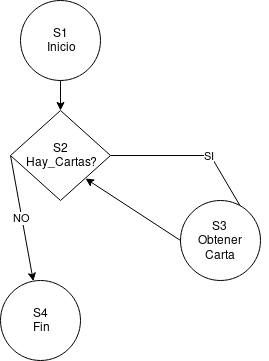
\includegraphics[scale=0.8]{figuras/getCartas.png}
		\caption{Grafo de caminos de la función.}
	\end{figure}

\begin{table}[htb]
\centering
\begin{tabular}{|l|l|l|}
\hline
\multicolumn{3}{|c|}{Devuelve una lista con las cartas en mano del jugador} \\ \hline
\multicolumn{3}{|c|}{public int getPuntuación()} \\ \hline
Cartas del jugador & Camino de la ejecución (estados) & Resultado \\ \hline	
C1 & S1, S2, S3, S4 & C1 \\ \hline
 \end{tabular}
 \caption{Entorno de prueba de la función.}
\label{}
\end{table}

Basta con una ejecución de la función porque si el jugador tiene solo una carta en la mano se prueban todos los caminos posibles del grafo.

Para las más complejas de la lógica como la función lanzarCarta de EstadoPartida y la función siguienteRonda se han realizado pruebas de caja negra para comprobar el correcto funcionamiento ya que son las funciones más importantes de la lógica del guiñote.

Para la función lanzarCarta las pruebas se realizan para los casos donde ya no queden cartas en el mazo (ronda de arrastre), debido a que antes del arrastre no existen restricciones en las cartas que se pueden tirar. Se separan las pruebas en dos: las pruebas para una partida de uno contra uno al segundo jugador tiene que lanzar una carta y las pruebas para el tercer jugador en lanzar cuando la partida es dos contra dos. No se han realizado pruebas para el primer jugador en lanzar ya que no tiene restricciones ni al cuarto ya que el código ejecutado es el mismo que para el tercer jugador.

\begin{center}
    \begin{tabular}{ | p{10cm} | p{5cm} |}
    \hline
\multicolumn{2}{|p{14cm}|}{Lanza la carta c por el Jugador "jugador". Si no es su turno, no posee dicha carta o incumple alguna de las reglas del guiñote, lanza una excepción.} \\ \hline
\multicolumn{2}{|l|}{public EstadoPartida lanzarCarta(String jugador, Carta c)} \\ \hline
{Casos durante la ronda de arrastre (2º jugador)} & Resultado \\ \hline
Lanza una carta de un palo diferente al inicial teniendo del mismo palo & Lanza excepción CartaIncorrecta \\ \hline
Lanza una carta del mismo palo al inicial pero de valor inferior teniendo una carta de valor superior y mismo palo al inicial & Lanza excepción CartaIncorrecta \\ \hline
Sin tener cartas del palo de la carta inicial, lanza una carta de un palo cualquiera teniendo triunfo & Lanza excepción CartaIncorrecta \\ \hline
Lanza una carta superior del mismo palo al inicial & Se añade la carta a la lista de cartas en el tapete \\ \hline
Lanza una carta inferior y del mismo palo a la inicial sin tener en la mano una superior del mismo palo & Se añade la carta a la lista de cartas en el tapete \\ \hline
Sin tener cartas del palo incial, lanza una carta del palo del triunfo & Se añade la carta a la lista de cartas en el tapete \\ \hline
Sin tener cartas del palo inicial o del palo del triunfo, lanza una carta cualquiera & Se añade la carta a la lista de cartas en el tapete \\ \hline
Casos durante la ronda de arrastre (3º jugador) & Resultado \\ \hline
Lanza una carta de un palo diferente al inicial teniendo del mismo palo & Lanza excepción CartaIncorrecta \\ \hline
Con obligación de matar(el compañero no tiene la carta con mayor valor), lanza una carta que no mate teniendo una carta de valor superior y mismo palo al inicial que mata al rival & Lanza excepción CartaIncorrecta \\ \hline
Con obligación de matar(el compañero no tiene la carta con mayor valor) y sin tener carta del palo inicial, lanza una carta que no mate teniendo triunfo & Lanza excepción CartaIncorrecta \\ \hline
Habiendo matado el rival sin triunfo, lanza una carta superior del mismo palo al inicial & Se añade la carta a la lista de cartas en el tapete \\ \hline
Habiendo matado el rival sin triunfo, lanza triunfo para matar & Se añade la carta a la lista de cartas en el tapete \\ \hline
Habiendo matado el compañero y sin tener del palo incial, lanza una carta de un palo cualquiera & Se añade la carta a la lista de cartas en el tapete \\ \hline

    \end{tabular}
    
\end{center}


Para la función siguienteRonda se ha probado cada caso donde un jugador diferente ganaba y se ha comprobado que sumaba los puntos correspondientes al equipo que ganaba. Además se ha verificado que tras la última baza si se alcanzaban los 100 puntos por parte de un equipo se daba por finalizada la partida y en caso de no alcanzarse se daba comienzo a la partida de vueltas.

\begin{table}[htb]
\begin{center}
\begin{tabular}{| p{7cm} | p{7cm} |}
\hline
\multicolumn{2}{|c|}{Asigna el turno y puntuación de las cartas del tapete de cada ronda al ganador de la ronda} \\ \hline
\multicolumn{2}{|l|}{public EstadoPartida siguienteRonda()} \\ \hline
Casos (4 jugadores) & Resultado \\ \hline
   	
Se ejecuta la función habiendo lanzado carta los tres primeros jugadores & Lanza excepción RondaNoAcabada \\ \hline
Se ejecuta sin que ningún jugador lance triunfo ni supere al primer jugador & Turno==0 ganadorUltimaRonda==0 
Puntuación j1 igual a la suma del valor de las cartas 
Puntuación j1 == Puntuación j3 \\ \hline
El jugador 2 mata con una carta superior & Turno==1 ganadorUltimaRonda==1
Puntuación j2 igual a la suma del valor de las cartas
Puntuación j2 == Puntuación j4 \\ \hline
El jugador 3 mata con un triunfo después de que el jugador 2 haya matado & Turno==2 ganadorUltimaRonda==2
Puntuación j1 igual a la suma del valor de las cartas
Puntuación j1 == Puntuación j3 \\ \hline
El jugador 4 mata con un triunfo superior después de que el jugador 3 haya matado & Turno==3 ganadorUltimaRonda==3
Puntuación j2 igual a la suma del valor de las cartas
Puntuación j2 == Puntuación j4 \\ \hline
En la última baza el jugador 4 mata con un triunfo superior después de que el jugador 3 haya matado sin superar los 100 puntos & Turno==3 ganadorUltimaRonda==3
Puntuación j2 igual a la suma del valor de las cartas
Puntuación j2 == Puntuación j4
deVueltas==1 \\ \hline
En la última baza el jugador 4 mata con un triunfo superior después de que el jugador 3 haya matado superando así los 100 puntos & Lanza excepción PartidaFinalizada \\ \hline

 \end{tabular}
 \caption{Pruebas de la función siguienteRonda().}
\label{}
\end{center}
\end{table}

Al tratarse de un videojuego, es difícil abordar todos las posibles situaciones de la partida, por lo que para probarlo, se hace el trabajo similar al de un tester, donde juega partidas y fuerza situaciones que se salen de lo normal para comprobar el comportamiento de la partida. Cuando se detecta algún bug, se notifica a través de un issue en GitHub para que el equipo causante del mismo lo solucione.



\subsubsection*{Progreso y Divergencias frente a la planificación inicial}

Para la primera iteración era necesario realizar una demostración al cliente de una versión funcional el juego del guiñote. Se ha realizado una versión básica funcional jugable a través de interfaz. Sin embargo, se ha dejado para la segunda iteración el requisito de cambio de dispositivo y de personalización del juego principalmente. Además, se garantizó que el modo espectador debía estar implementado. Sin embargo, no está desarrollado plenamente. La situación actual de la implementación de dicho requisito está casi terminada, a falta de la integración con la comunicación entre capas y las pruebas correspondientes.

En el primer plan de gestión se especificó que tanto el matchmaking y como la web dinámica deberían estar avanzados para la primera iteración. En cuanto a la web dinámica, faltan bastantes vistas y funcionalidades básicas debido a la sobre carga de trabajo que han sufrido los equipos de backend y frontend. Ambos equipos se centraron en obtener las funcionalidades básicas del juego dejando de lado el resto de aspectos. Si bien es cierto que ya se ha alcanzado un tercio del total, mientras que el objetivo en esta primera iteración era de la mitad.

En cuanto a la capa de persistencia y la capa de acceso de datos, el equipo de bases de datos ha cumplido el diagrama de Gantt establecido, exceptuando la implementación del acceso a datos relacionado con los torneos, que estaba planificado para la primera iteración y se debe alargar a la segunda, sin suponer ningún problema de dependencias con el resto de componentes del sistema y que no se estima muy costosa. También se puede comentar que, en lo que respecta al diseño de la base de datos, se requirió algo menos tiempo del estimado (se finalizó con una semana de antelación), mientras que el diseño del acceso a datos requirió más tiempo del estimado por lo que fueron compensados, cumpliendo bastante bien la planificación inicial.

En cuanto a la 2ª iteración, se ha conseguido implementar el resto de requisitos en su plenitud. De los cuales, los más importantes eran el matchmaking, torneos, espectadores, permitir el cambio de dispositivo y la incorporación de la inteligencia artificial. El más problemático ha sido implementar la posibilidad de los torneos, ya que el equipo se ha enfrentado a diferentes problemas de diseño relacionados con el abandono de jugadores. La integración de la inteligencia artificial también ha resultado ser problemática ya que respondía practicamente de manera instantánea y el jugador no podía ver la carta que ésta había lanzado.
\\
Debido a los problemas comentados anteriormente las horas de trabajo se incrementas considerablemente. Además, habría que sumarle los problemas realacionados al despliegue y la latencia de la red que aparece y como lidiar con este nuevo problema.

\subsubsection*{BackEnd}
El equipo ha cumplido el diagrama de Gantt en el apartado de implementación de lógica del juego. Si bien es cierto que se ha logrado con un retraso de media semana. Puesto que el equipo se centró en la implementación de la lógica la parte de desarrollo de la web dinámica no ha cumplido el calendario impuesto al comienzo del proyecto y arrastra un leve retraso que deberá ser compensado en la segunda iteración. El retraso se debe a la gran cantidad de trabajo asignado en la planificación inicial, muy superior a la capacidad del equipo.

Debido a las divergencias entre las horas de implementación reales y las estimaciones iniciales, el equipo ha decidido realizar un registro y posteriormente un estudio de las horas empleadas en el desarrollo del proyecto. El equipo ha realizado 349 horas de trabajo, de las cuales 106 se han invertido en tareas de gestión, una cifra muy superior a establecida en la estimación inicial. También cabe destacar las 33 horas de realización de pruebas y corrección de errores, que deberían asegurar la calidad del proyecto. En cuanto a las estimaciones sobre los diferentes componenetes, la implementacion del juego y su comunicación, junto con el desarrollo de la web dinámica están realizadas de forma precisa, completando las horas asignadas. Sin embargo, los componentes de la base de datos y las vistas de la web se han sobredimensionado ligeramente, por lo que el equipo ha tenido que realizar menos trabajo del especificado. 

Como se ha explicado anteriormente, como respuesta a los problemas de divergencias de horas de trabajo frente a la planificación se realizó una reestructuración de los equipos de trabajo que afectó al equipo de Inteligencia Artificial. Se decidió incorporar a los nuevos miembros en este equipo y no a otras tareas porque era el único que todavía no había comenzado a trabajar y, por tanto, la reestructuración no afecta al rendimiento del equipo de trabajo como ocurriría si fuesen añadidos a mitad (tal y como se explica en el libro Mythical Man-month cuyo tema principal es la idea de \textit{'adding manpower to a late software project makes it later'} \cite{libroMMM}.)


\subsection{Cierre del proyecto}
\label{Cierre del proyecto}
Los procesos de control no se han llevado a cabo tal y como estipulaba el primer plan de gestión. Ya que el director del proyecto no se ha coordinado con los responsables de grupo. Sin embargo a nivel local, los responsables de grupo si han dirigido y organizado sus respectivos grupos. Además no se ha producido ninguna situación que requiera de mediación ni necesidad de int
\subsubsection{Comparación estimaciones iniciales}
En la fase inicial del proyecto se realizó una estimación inicial del coste de 630 horas de desarrollo de software y 170 horas en gestión del proyecto, de la calidad del software y de las configuraciones. Un total de 800 horas, de las cuales se han llevado a cabo 778 horas, un 97\%. A pesar de que la estimacion global se haya cumplido, una análisis más fino de la distribución de las horas revela unas conclusiones diferentes.

\begin{table}[htb]
\centering
\begin{tabular}{|l|l|l|l|}
\hline
\multicolumn{4}{|c|}{Distribución de las horas del proyecto en diferentes agrupaciones} \\ \hline
	Agrupacion & Estimacion & Horas invertidas & Porcentaje cumplido\\ \hline
	Desarrollo del juego & 128 h & 160 h & 125\%\\ \hline
	Pagina web & 140 h & 82 h & 58\% \\ \hline
	Base de datos & 122 & 88 h & 72\%\\ \hline
	Despliegue & 10 h & 20 h & 200\%\\ \hline
	Implementacion IA & 85 h & 64 h & 75\% \\ \hline
	MatchMaking & 35 h & 26 h & 74\% \\ \hline
	Gestión & 95 h & 141 h & 148\% \\ \hline
	Gestión de configuraciones & 31 h & 20 h & 64\% \\ \hline
	Aseguramiento de la calidad & 44 h & 136 h & 300\% \\ \hline
	Integración & 0 h & 22 h & -\% \\ \hline
 \end{tabular}
 \caption{Distribucion de las horas por tipo de actividad}
\label{}
\end{table}

Como se puede apreciar en la tabla, la distribución de las horas estimadas y la de las invertidas son muy diferentes. Estas divergencias entre la estimación y los resultados finales se deben a la falta de experiencia en la realización de proyectos de esta magnitud, el desconocimiento de la dificultad del aseguramiento de la calidad en juegos online y algunos errores en el diseño del proyecto. Como por ejemplo la subestimación de los componentes de comunicación y sincronización.

A nivel individual el equipo ha trabajado de forma uniforme y repartiendo la carga de trabajo. La división de los integrantes del equipo en grupos de trabajo se ha llevado a cabo de forma efectiva y muestra de ello es la siguiente tabla que recoge un resumen del trabajo de cada miembro.

\begin{table}[htb]
\centering
\begin{tabular}{|l|l|l|}
\hline
\multicolumn{3}{|c|}{Distribución de las horas del proyecto por persona} \\ \hline
	Nombre & Horas trabajadas & Actividad principal \\ \hline
	Javier & 106 h & Gestor de mensajes y MatchMaking \\ \hline
	Marius & 116 h & Implementación de la lógica del juego y servlets \\ \hline
	Sergio & 128 h & Diseño de la base de datos y representación del problema de la IA \\ \hline
	Carlos & 108 h & Interfaz y vistas web \\ \hline
	Víctor & 117 h & Web dinámica y representación de la lógica del juego \\ \hline
	Julia  & 123 h & Diseño de la base de datos y análisis de la IA \\ \hline
	Ignacio & 79 h & Pruebas y lógica del juego \\ \hline
 \end{tabular}
 \caption{Distribucion de las horas por persona}
\label{}
\end{table}

\subsubsection{Lecciones aprendidas sobre herramientas y tecnologías}
La experiencia con IntelliJ, el entorno con el que se ha desarrollado el sistema, ha sido positiva en su totalidad. Gracias a su plena integración con Git, no hace falta realizar ninguna acción externa a la aplicación. Sin embargo, conforme el proyecto se iba desarrollando, los problemas de configuración del mismo aumentaban debido a las dependencias y la organización interna del mismo. Ésto no habría pasado si se hubiera configurado con Maven o Graddle en vez de hacerlo manualmente.
\\
En cuanto a la tecnología Phaser, la experiencia ha resultado ser positiva. Se trata de un software fácil de usar por lo que su aprendizaje no ha sido del todo costoso. Además, gracias a la comunidad disponible se han podido resulver las dudas sin problema alguno. La utilización de WebSockets para el paso de mensajes ha resultado más costosa ya que se deben tratar las desconexiones de los jugadores de manera individual. Habría sido más efectivo tratar de utilizar una teconología basada en eventos, por ejemplo.
\\
El software utilizado para los diagramas ha sido StarUML. Éste ha ofrecido una experiencia neutra. Cumple en todos sus aspectos pero el tener la versión gratuita hace que cada vez que sea ejecutado apareza el mensaje de compra.
\\
Todo el proyecto salvo la interfaz ha sido implementada en Java ya que era una tecnología con la que ya se ha trabajado pero en retrospectiva se considera que se podría haber ahorrado tiempo utilizando un lenguaje de programación menos verboso como Kotlin (por compatibilidad con la JVM), Go, Python, Javascript, etc, que además ofrecen facilidades para la gestión de dependencias, CI/CD y escalabilidad horizontal en Kubernetes por ejemplo, lo que sería especialmente útil para gestionar grandes volúmenes de partidas a la vez.